\chapter{A Few More Classifiers}
\label{ch:more-classifiers}

\begin{marginfigure}[2.0cm]
    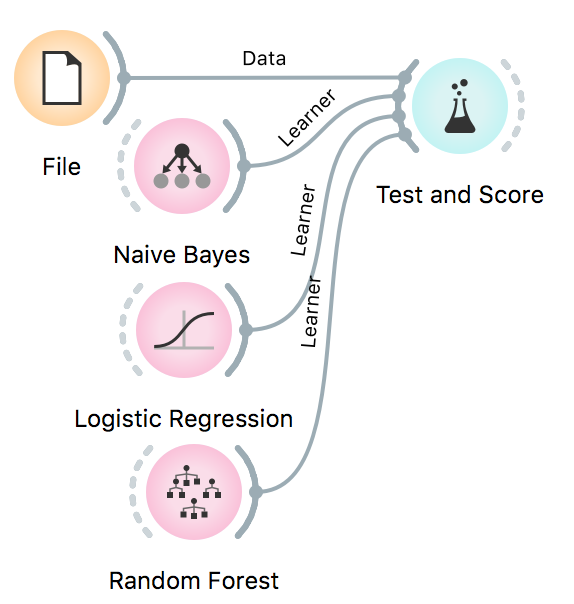
\includegraphics[width=\linewidth]{workflow1.png}
\end{marginfigure}

We have ended the previous lesson with cross-validation and classification trees. There are many other, much more accurate classifiers. A particularly interesting one is Random Forest, which averages across predictions of hundreds of classification trees. It uses two tricks to construct different classification trees. First, it infers each tree from a sample of the training data set (with replacement). Second, instead of choosing the most informative feature for each split, it randomly selects from a subset of most informative features. In this way, it randomizes the tree inference process. Think of each tree shedding light on the data from a different perspective. Just like in the wisdom of the crowd, an ensemble of trees (called a forest) usually performs better than a single tree.

Another popular classifier is logistic regression.\marginnote{Logistic regression is a classification, not a regression method. It is called regression because it is methodologically similar to linear regression.} In this model, each variable has its weight or importance. Logistic regression computes weights of each variable during the training phase. For prediction, it simply multiplies the weight of the variable with its value, computes the total sum and log transforms it into probability.

\begin{marginfigure}
    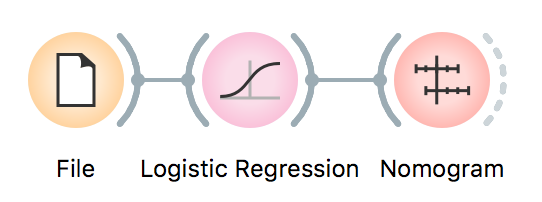
\includegraphics[width=\linewidth]{workflow2.png}
\end{marginfigure}

We can use Nomogram to observe the importance of variables in a model and their weights. The variables in the plot are ranked and the length of the line corresponds to their importance in the model.

\begin{figure}
    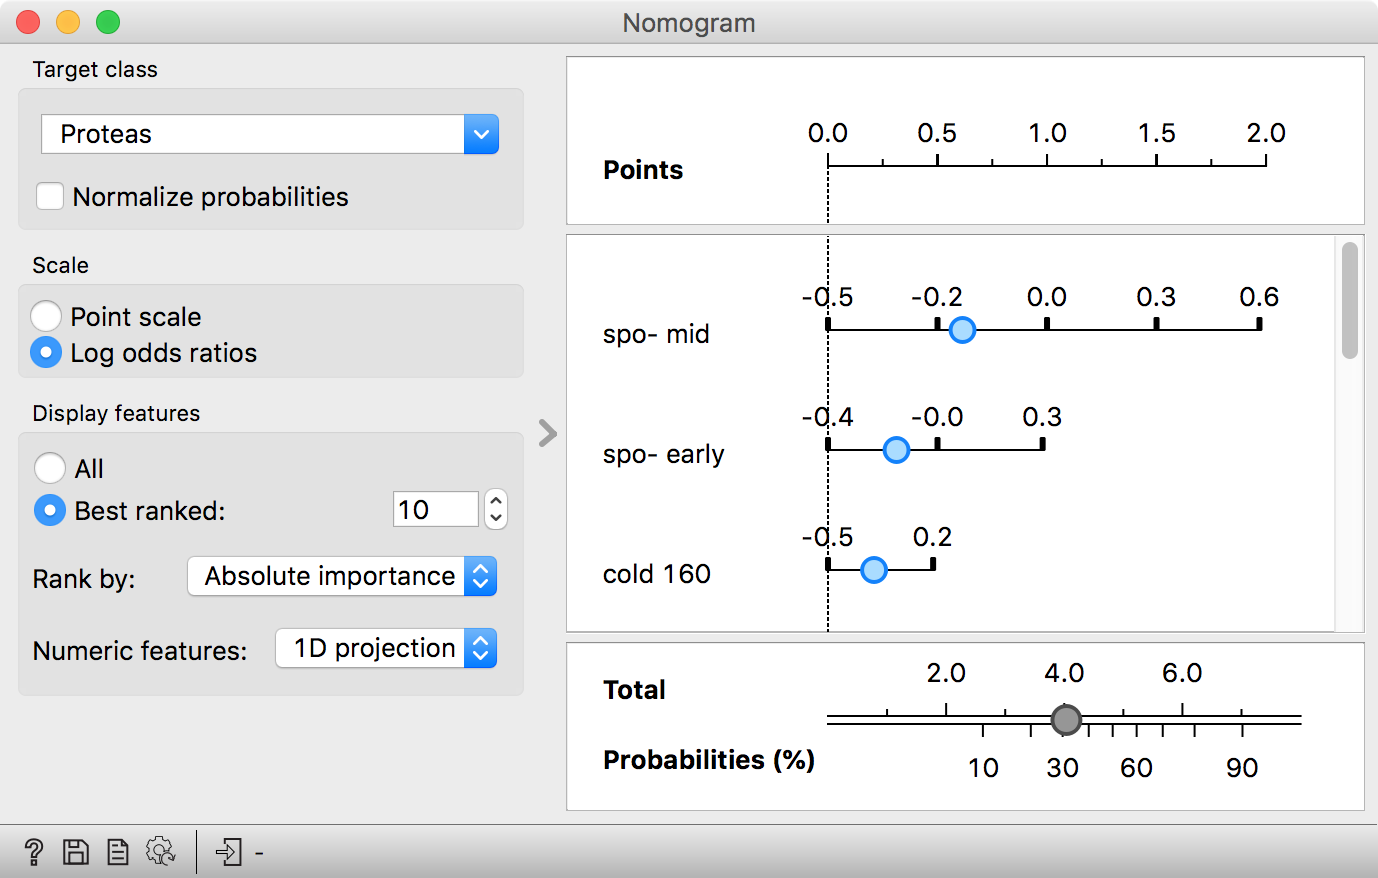
\includegraphics[scale=0.6]{nomogram.png}
    \label{fig:nomogram}
\end{figure}
